\documentclass{beamer}
\usetheme{Boadilla}
\makeatletter
\def\th@mystyle{%
    \normalfont % body font
    \setbeamercolor{block title example}{bg=orange,fg=white}
    \setbeamercolor{block body example}{bg=orange!20,fg=black}
    \def\inserttheoremblockenv{exampleblock}
  }
\makeatother
\theoremstyle{mystyle}
\newtheorem*{remark}{Remark}
\newtheorem*{task}{Task}
\newtheorem*{idea}{Idea:}
\newtheorem*{dood}{}
\usepackage{bbm}
\usepackage{tikz-cd,mathtools}
\usepackage{cancel}  
\newcommand{\A}{\mathbb{A}}
\newcommand{\N}{\mathbb{N}}
\newcommand{\Z}{\mathbb{Z}}
\newcommand{\Q}{\mathbb{Q}}
\newcommand{\R}{\mathbb{R}}
\newcommand{\C}{\mathbb{C}}
\newcommand{\f}{\mathfrak{f}}
\newcommand{\F}{\mathbb{F}}
\newcommand{\g}{\mathfrak{g}}
\newcommand{\K}{\mathbb{K}}
\renewcommand{\l}{\mathfrak{l}}
\newcommand{\p}{\mathfrak{p}}
\renewcommand{\P}{\mathfrak{P}}
\newcommand{\PP}{\mathbb{P}}
\mode<presentation>{}
\usepackage{amscd}
\tikzcdset{ampersand replacement=\&}
\usepackage{tikz-cd}
\tikzcdset{ampersand replacement=\&}
\usepackage{tikz}
\usepackage{mathtools}
\usepackage{array}
\usepackage[utf8]{inputenc}
\usepackage[T1]{fontenc}
\usepackage{textcomp}
\usepackage[english]{babel}
\usepackage{amsmath, amssymb}
\usepackage[mathscr]{euscript}
\usepackage{subcaption}
\usepackage{graphicx}
\usepackage{listings}
\usepackage{xcolor}
\graphicspath{ {./} }
\begin{document}
\title{A Benchmark for Interpretability Methods in DNNs}
\subtitle{(Google Brain)}
\author{Sam Laing }
\institute{University of Tuebingen}
\date{\today}
\begin{frame}
\titlepage
\end{frame}
\begin{frame}
	\frametitle{A Bit of Background}
	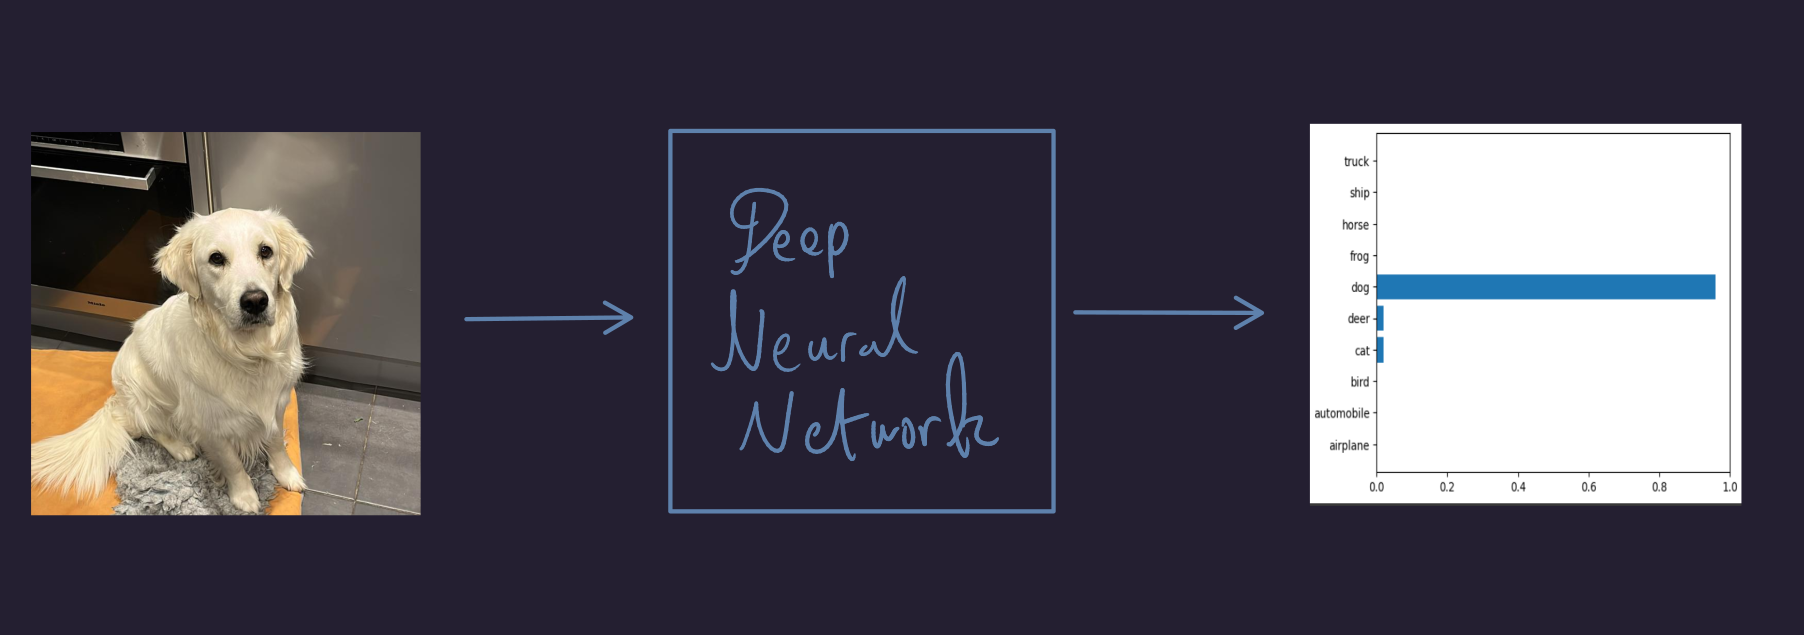
\includegraphics[width = 11cm, height = 5cm]{dog_net2.png} \pause
	\begin{itemize}
		\item Deep image classification: "features" = pixels .\pause
		\item Interpretability methods $\to$ help engineer understand their model\pause
		\item Ostensibly. But are they really doing anything?
		\item Interpretability method A $>$ Interpretability method B??\pause
		\item If only there was a benchmarking framework to do this...
	\end{itemize}
\end{frame}


\begin{frame}
	\frametitle{Included Interpretability Methods}
	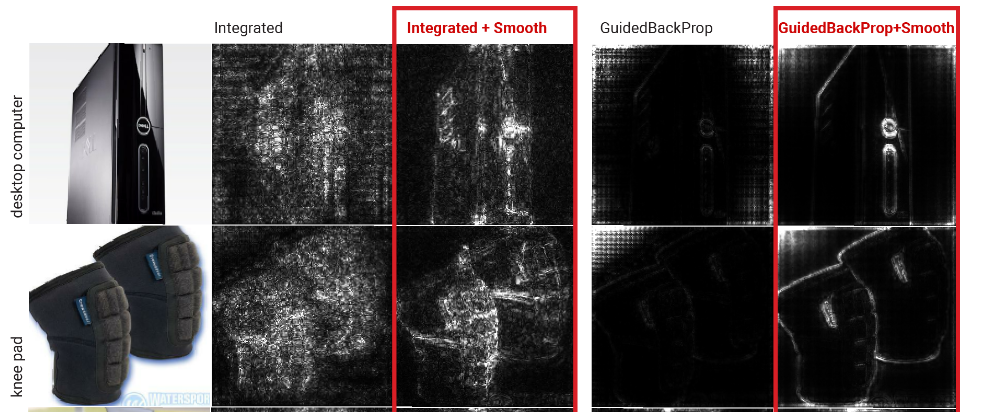
\includegraphics[width=10cm, height=5cm]{compareSGBP.png}

	\begin{itemize}
	
	\item Gradients (sensitivity heatmaps) $e = \partial_{x_i} f_c(x) $ \pause

	\item Guided Backprop (sort of a tidied up sensitivity map). Keep positives in ReLU \pause
	\item Integrated Gradients
	
	\end{itemize}
\end{frame}

\begin{frame}
    \frametitle{Included Interpretability Methods: Ensembling in a Nutshell}
    \begin{columns}[T] % Align columns at the top
        \begin{column}{0.7\textwidth}
            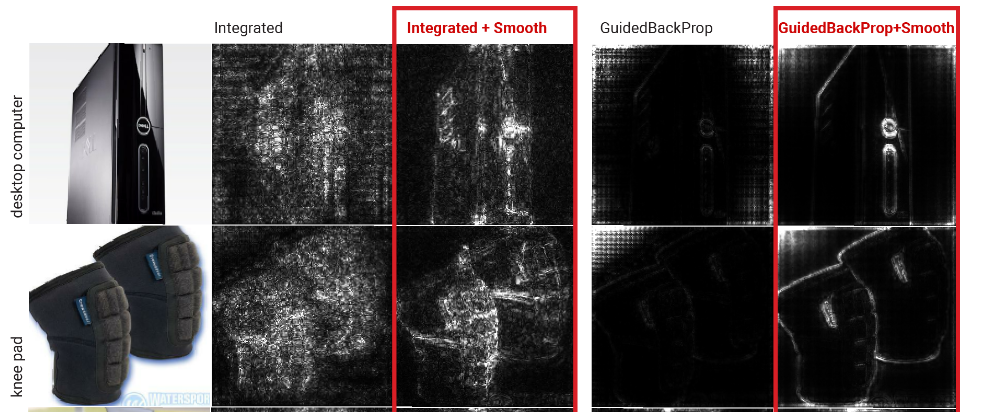
\includegraphics[width=1.0\textwidth, height=4cm]{compareSGBP.png}
        \end{column}
        \begin{column}{0.3\textwidth}
		Smilkov's "Smoothgrad" paper (2017): \\
		"Reduce noise by adding noise"
        \end{column}
    \end{columns}
    \begin{itemize}
        \item Inject inputs with Gaussian noise consider mean/variance of outputs \pause
        \item $\eta_i \sim N(0, \sigma ^2 I)$ $i\in \{1,\ldots, J\} $ \pause
	\item SmoothGrad (SG) $e = \sum_{i=1}^{J} {f_{c}( x + \eta_i) }$ \pause
	\item VarGrad (VAR) $e = \text{Var}( \{ {f_{c}(x + \eta_i)} \}_{i=1}^J) $ \pause
	\item SmoothGrad Squared (SG-SQ) $e = \sum_{i=1}^{J} {f_{c}( x + \eta_i)^{2} }$\pause
    \end{itemize}
$\to$Apply attribution/interpretability methods to these statistics
\end{frame}


\begin{frame}
	\frametitle{ROAR (RemOve And Retrain)}
	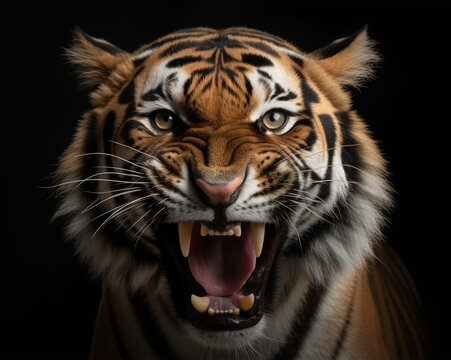
\includegraphics[height=5.5cm, width=8cm]{tiger.png}\\
\end{frame}


\begin{frame}
	\frametitle{The Idea Behind ROAR}
	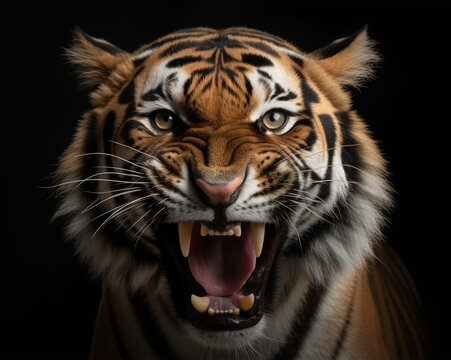
\includegraphics[height=5.5cm, width=8cm]{tiger.png}\\
	Start with trained classifier $f$\\ \pause

	$\forall $  method, $\forall $ image $\in$ dataset, sort pixels by ranked importance. \\ \pause 
	

	So $(e_j)_{j=1}^{D}$ of pixel coordinates $\forall $ image in dataset. $\implies ( (e_j^{(n)})_{j=1}^D )_{n=1}^N $
\end{frame}
\begin{frame}
	\frametitle{The idea behind ROAR}

	for $j \in \{0, 10, \ldots,100\} $, replace the top j\% ranked pixels with the per channel mean  $\forall $ image and retrain.
	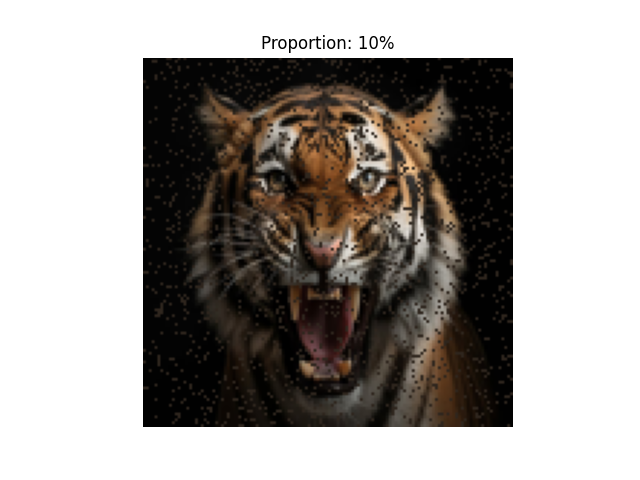
\includegraphics[height=8cm, width=10cm]{tiger0.1.png}

\end{frame}
\begin{frame}
	\frametitle{The idea behind ROAR}
	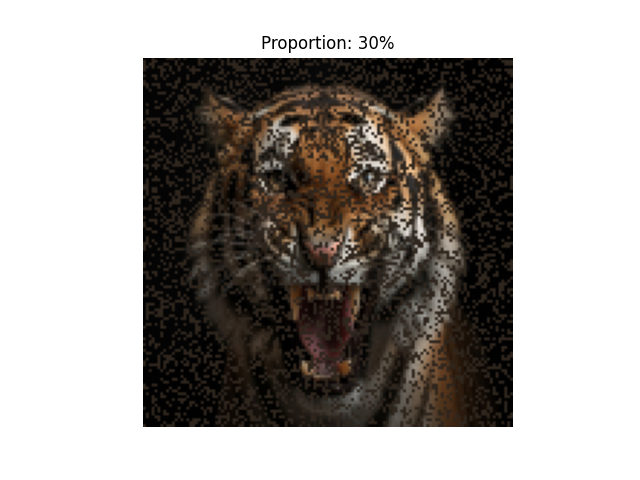
\includegraphics[height=8cm, width=10cm]{tiger0.3.png}

\end{frame}

\begin{frame}
	\frametitle{The idea behind ROAR}
	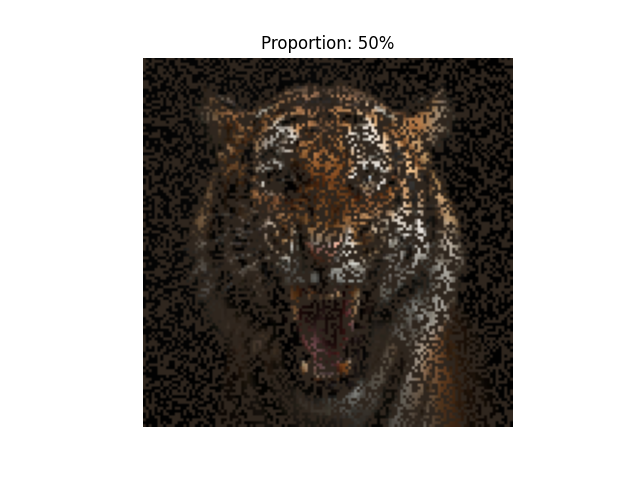
\includegraphics[height=8cm, width=10cm]{tiger0.5.png}

\end{frame}

\begin{frame}
	\frametitle{The idea behind ROAR}
	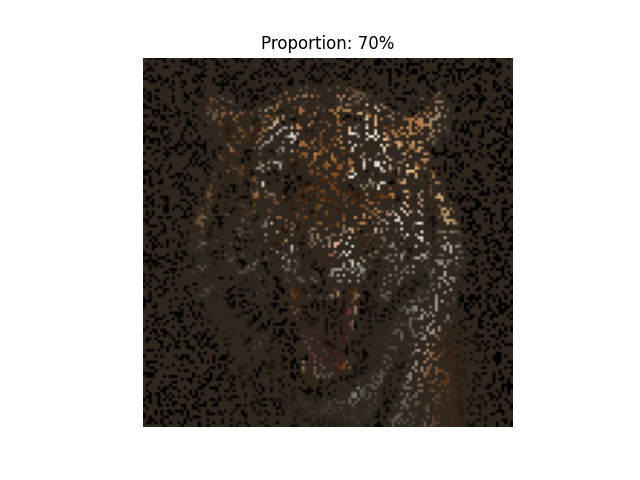
\includegraphics[height=8cm, width=10cm]{tiger0.7.png}

\end{frame}


\begin{frame}
	\frametitle{The idea behind ROAR}
	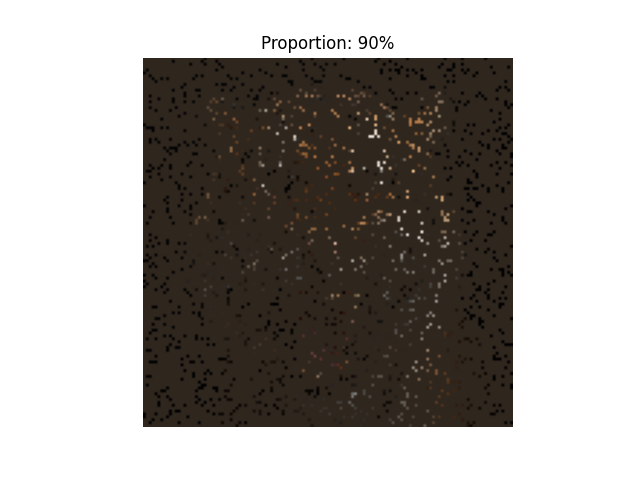
\includegraphics[height=8cm, width=10cm]{tiger0.9.png}

\end{frame}
\begin{frame}
	\frametitle{The idea behind ROAR}
	\begin{itemize}
		\item Effect of having dropped the "most informative pixels" as determined by each interpretability method.
		\item Investigate how much their removal from the training process effects accuracy.		
		\item Also a no-retraining variant
	\end{itemize}
\end{frame}
\begin{frame}
	\frametitle{To Retrain Or not To Retrain}
	\begin{itemize}
	\item No retraining  $\implies p_{\ \text{train}} \neq p_{ \ \text{test}}$ ... $\rightarrow \ \leftarrow$ in ML \pause
	\item Paper therefore argues it is necessary \pause
	\end{itemize}
	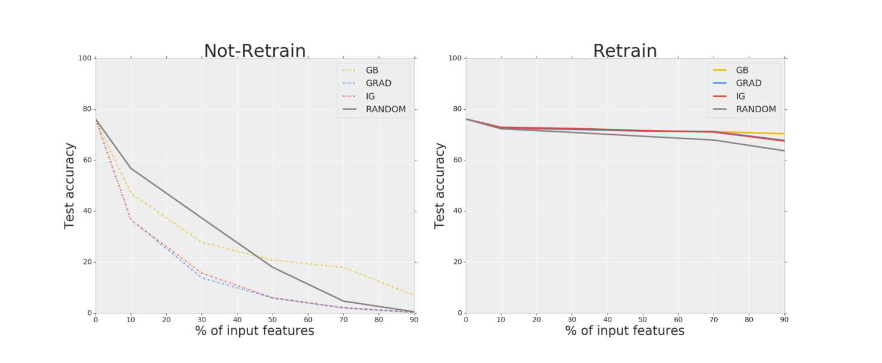
\includegraphics[width=12cm, height=5cm]{retrain_vs_not.png}\pause
	\begin{itemize}
	\item Paper does some validation with synthetic data but unconvincing.
	\end{itemize}
\end{frame}

\begin{frame}
	\frametitle{An Outline of the Experiment}
	Really just a refinement of above.
	\begin{itemize}
		\item ResNet50 classifier: Imagenet, Birdsnap and Food 101\pause
		\item Random pixel selection and Sobel Edge filter benchmarks.\pause
		\item  New train and test sets $\forall  \ j \in \{0,10,30,50,70,90\} $\pause
		\item Each model retrained 5 times $\forall $ method (DNN training is noisy) 
	\end{itemize}
\end{frame}

\begin{frame}
	\frametitle{ROAR in Action}
	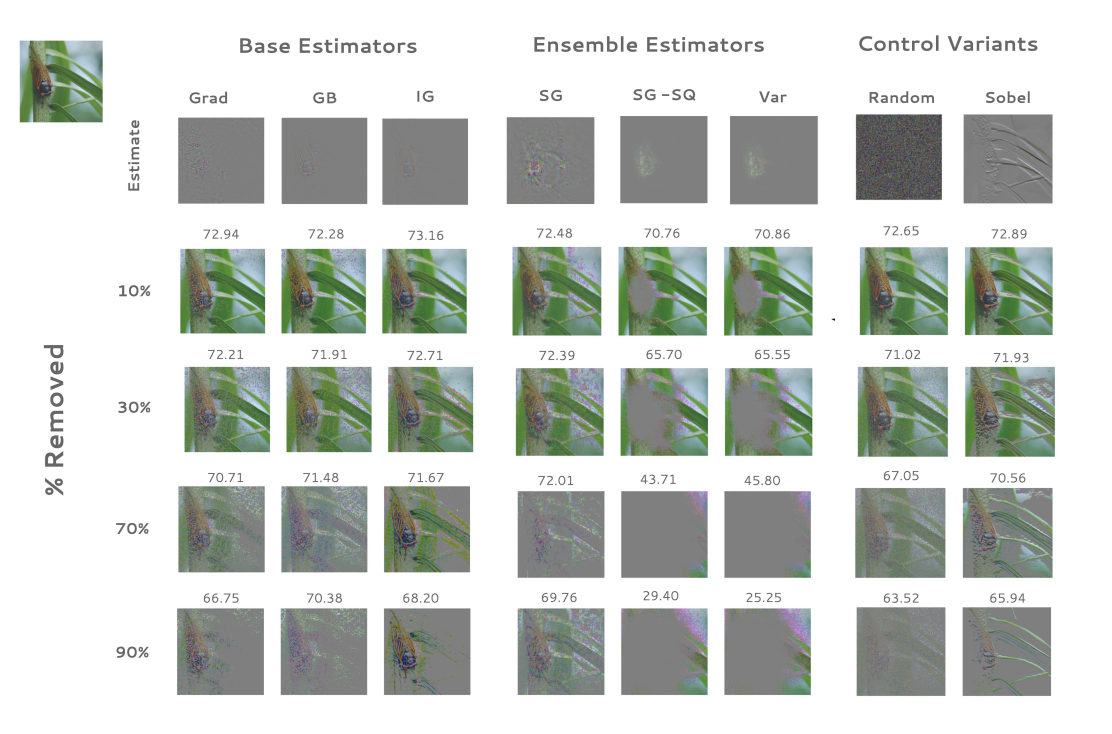
\includegraphics[height=7.2cm, width=10cm]{ROAR_methods.png}\\ \pause
	Initial Imagenet accuracy: $\sim78$ \% ... \pause Paper is from 2018!
\end{frame}

\begin{frame}
	\frametitle{ROAR in Action}
	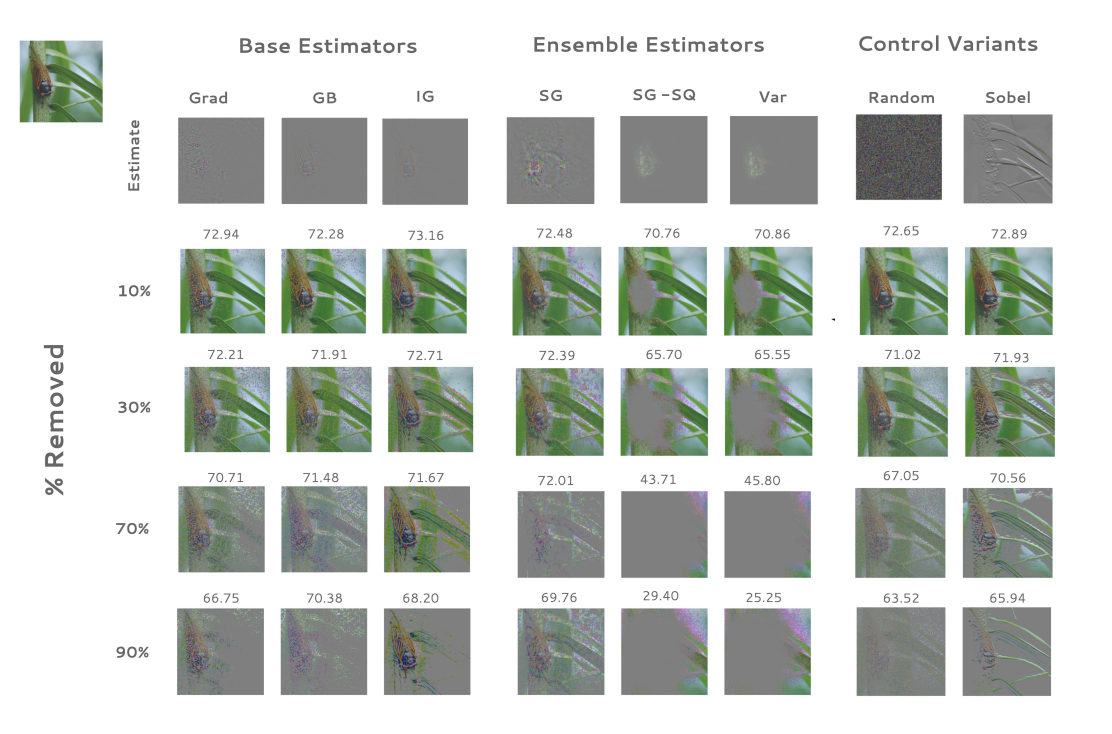
\includegraphics[height=7.2cm, width=10cm]{ROAR_methods.png}\\
	On average Replacing many pixels $\cancel{\implies}$ big decrease of predictive power! 

\end{frame}




\begin{frame}
	\frametitle{Results}
	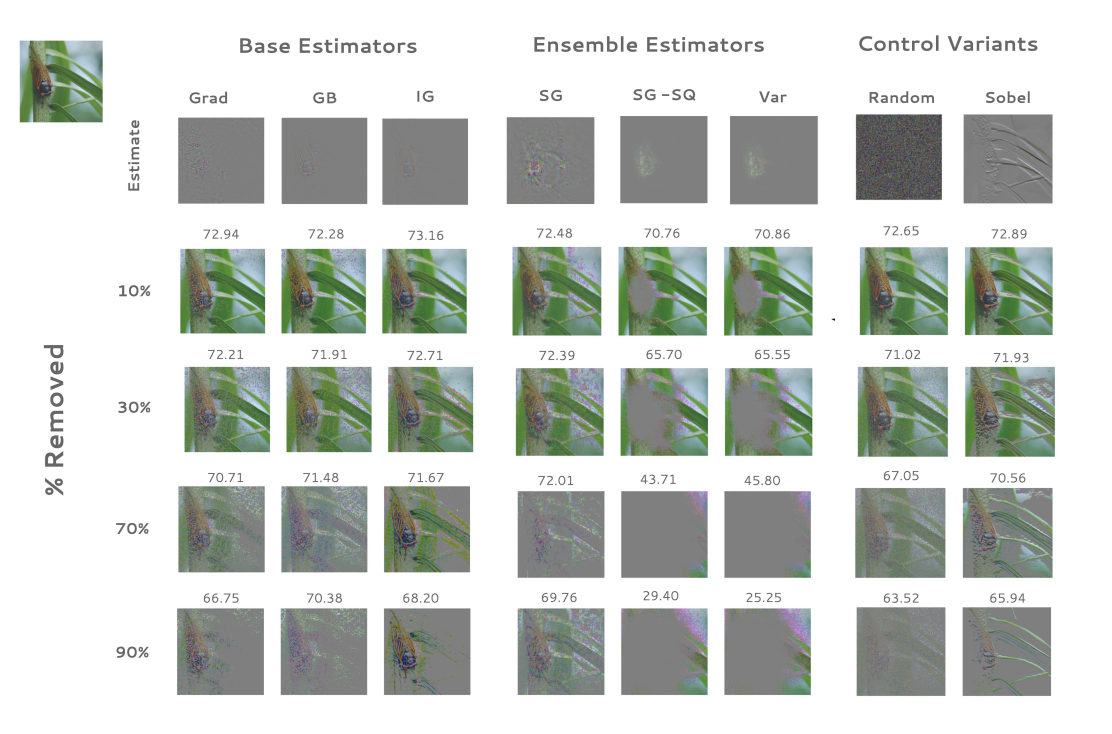
\includegraphics[height=7.2cm, width=10cm]{ROAR_methods.png}\\
	ImageNet, 90\% pixels randomly removed... still 63.52\% accuracy relative to the original 78.68\% \pause
\end{frame}

\begin{frame}
	\frametitle{Results}
	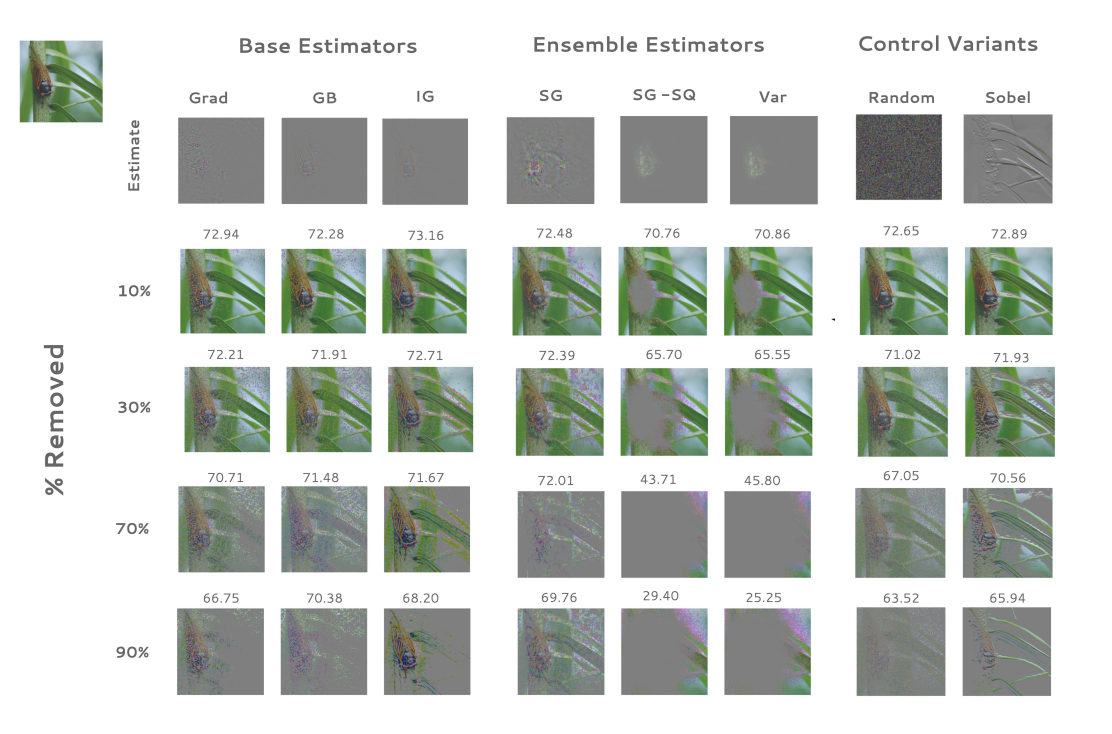
\includegraphics[height=7.2cm, width=10cm]{ROAR_methods.png}\\

	According to the paper, SG-SQ and VarGrad are the real heros 
\end{frame}

\begin{frame}
	\frametitle{Plots}
	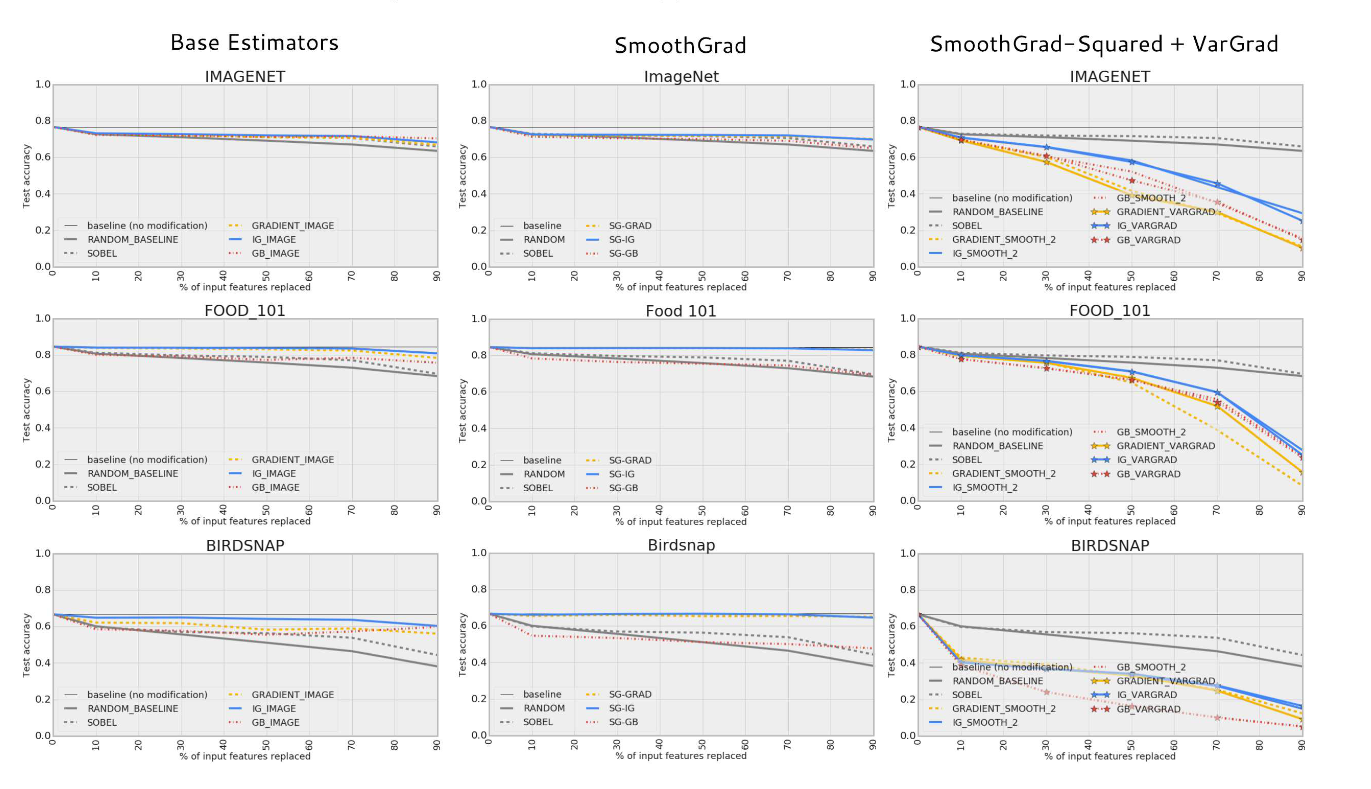
\includegraphics[width = 10cm, height=7.2cm]{all_the_plots.png}\\
	SG - SQ and VarGrad always outperformed... \pause
	\\
	But best method to wrap around changed

\end{frame}
\begin{frame}
	\frametitle{My Thoughts (Dummy Disclaimer!)}
	\begin{itemize}
	\item Why VAR and SG-SQ over Vanilla SG? \\ \pause 
	\item Variance captures more of the distribution's properties than mean?\\ \pause
	\item SG-SQ something of a middleground as unnormalized \\ \pause
	\end{itemize}
	\begin{align*}
		\text{SG-SQ:  } e_2 := \sum_{i=1}^{J} {f_{c_i} (x+\eta_i)^2} \quad &, \quad \text{SG:  } e := \sum_{i=1}^{J} {f_{c_i}(x+\eta_i)} \\
	\pause
		\implies \partial_{x_d} e_2 = 2 e . &\partial_{ x_d} e   \quad  \forall d
	\end{align*}
	Gradient of $e_2$ might encode more info since mean explicitely there
\end{frame} 
\begin{frame}
    \frametitle{A Few Possible Issues in the Approach}
    \begin{itemize}
	 \item Replace the top j pixels the mean.\pause
	
        \item Still conveys possibly useful information \pause
	\item "Missingness" not well defined for images \pause
    \end{itemize}
    \begin{minipage}{0.48\textwidth}
        \centering
        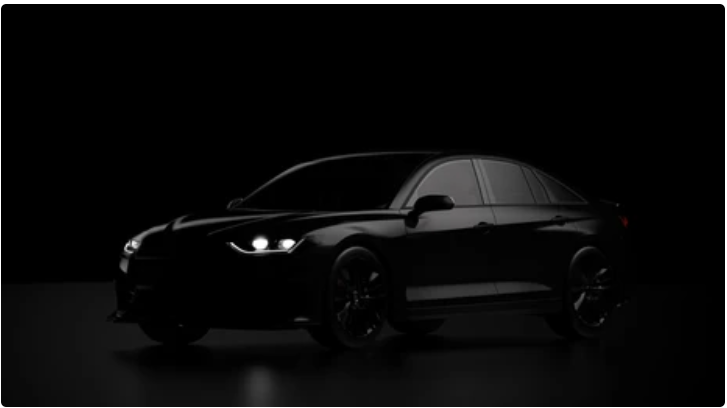
\includegraphics[width=\textwidth, height=3.5cm]{black_car.png}
    \end{minipage}
    \hfill
    \begin{minipage}{0.48\textwidth}
        \centering
        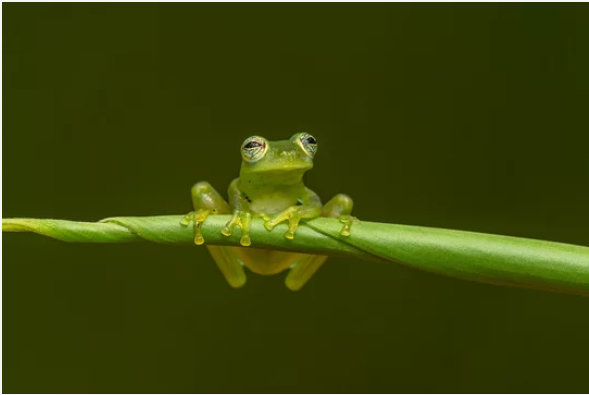
\includegraphics[width=\textwidth, height=3.5cm]{green_frog2.png}
    \end{minipage}
\end{frame}
\begin{frame}
	\frametitle{Another possible Issue}
	\begin{itemize}
	\item Cost! 
	\item More compute needed for big datasets \pause
	\item Retraining a large image classifier many times may be unfeasible  \pause
	\item Best depends on dataset \\
	\item Without retraining, you run into theoretical violations of ML!
	\end{itemize}
\end{frame}
\begin{frame}
\frametitle{Why I chose this paper}\pause
So many interpretability methods boast high performance: How to pick the right one? 
\\
Hard to find strong quantitative statements about explainability accuracy. \pause

\vspace{0.3cm}

    \textcolor{blue}{\textbf{\Large Did I like it?}} \pause
   
    \vspace{0.3cm}

    Yes and No! \\ \pause
    Quantitative framework and discovery are nice. \\ \pause
    Some of the details might need refinement \\ \pause
    Slightly limited number of techniques compared \\
    Paper used unclear notation and ommitted details at times
\end{frame}
\begin{frame}
	\frametitle{Questions?}
\end{frame}
\end{document}

